\chapter{Phương pháp tìm kiếm cục bộ giải bài toán tối ưu thời gian sống của mạng cảm biến không dây ngầm}
Giải thuật di truyền cùng với thuật toán heuristics đều là các phương pháp giải xấp xỉ, điều này đưa đến một ý tưởng mới để giải quyết bài toán: trong trường hợp có thể giải một pha nào đó của bài toán bằng thuật toán chính xác, liệu có thể cải thiện được lời giải của bài toán hay không?

Xét quá trình truyền nhận dữ liệu trong mô hình như sau:
\begin{figure}[H]
    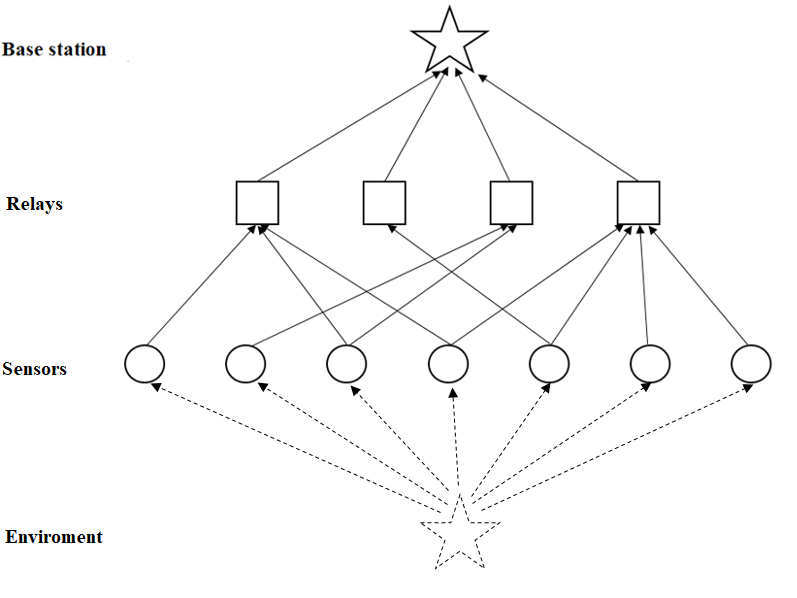
\includegraphics[width=\linewidth]{picture/lite_flow.png}
    \caption{Truyền nhận dữ liệu trong mạng}
\end{figure}
Nhìn vào hình vẽ trên, dễ dàng liên tưởng đến bài toán luồng trong mạng khi coi môi trường đặt cảm biến là một điểm phát giả và điểm thu là base station, khả năng thông qua của các cung source – sensor là 1, sensor - relay là 1, của các cung relay - base station là số sensor mà relay đó có thể kết nối. 
\\Dựa vào việc giải quyết bài toán luồng trong mạng với chi phí cực tiểu, ta có thể xác định được kết nối giữa các căp relay - sensor. Tuy nhiên với phương pháp này, trước đó ta cần biết được các vị trí đặt relay và mỗi relay kết nối với bao nhiên sensor để có được khả năng thông qua của cung.
\\Đề xuất giải thuật LSMF:
\begin{itemize}
    \item Sử dụng tìm kiếm cục bộ để xác định vị trí đặt relay và số sensor relay đó kết nối tới.
    \item Lượng giá lời giải bằng thuật toán luồng cực đại trong mạng với chi phí.
\end{itemize}
 \section{Tìm kiếm cục bộ}
 \textbf{Mã hóa lời giải}
 \\Lời giải của bài toán được mã hóa bởi vector: $k = (k_1, k_2,…, k_m)$.
\\Trong đó: 
\begin{itemize}
    \item $k_j$ là số sensor mà relay $j$ kết nối, $1 \leq j \leq m$
    \item $k_j \leq q_j ~\forall 1 \leq j \leq m$ 
    \begin{equation*}
        q_j = \sum_{i = 1}^n c_{ij} ~\forall 1 \leq i \leq n
    \end{equation*}
    \begin{itemize}
        \item[] $q_j$ là số sensor tối đa relay $j$ có thể kết nối
        \item[] $C$ là ma trận kết nối đã nêu trên
    \end{itemize}
    \item Tổng số sensor mà các relay kết nối tới đúng bằng số sensor trong mạng.
    \begin{equation*}
        \sum_{j = 1}^m k_j = n
    \end{equation*}
\end{itemize}
\textbf{Toán tử di chuyển}
\\Đề xuất sử dụng ba toán tử di chuyển:
\begin{itemize}
    \item Swap: chọn 2 chỉ số $i, j$ thỏa mãn $1 \leq i, j \leq m$, , trao đổi giá trị của $k_i, k_j$. 
    \item Transfer: chọn 2 chỉ số $i, j$ thỏa mãn $1 \leq i, j \leq m, k_i + k_j \leq q_i$, chuyển tất cả sensor từ relay $j$ sang relay $i$.
    \item Up – down: chọn 2 chỉ số $i, j$ thỏa mãn $1 \leq i, j \leq m, k_i > 0, k_j < q_j$, chuyển 1 sensor từ relay $i$ sang relay $j$.
\end{itemize}

\begin{figure}[h!]
    \centering
    \begin{subfigure}[b]{0.4\linewidth}
        \centering
        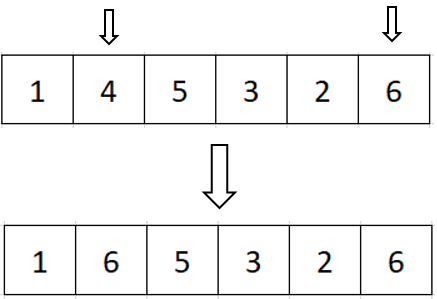
\includegraphics[width=0.8\linewidth]{picture/move1.png}
        \caption{Swap}
    \end{subfigure}
    \begin{subfigure}[b]{0.4\linewidth}
        \centering
      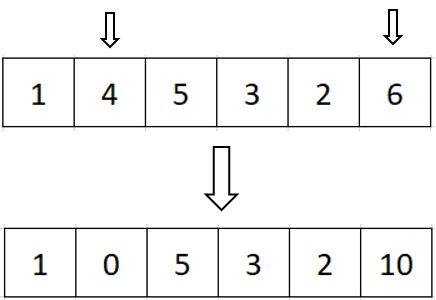
\includegraphics[width=0.8\linewidth]{picture/move2.png}
      \caption{Transfer}
    \end{subfigure}
    \begin{subfigure}[b]{0.4\linewidth}
        \centering
        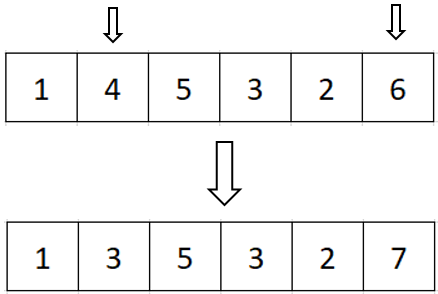
\includegraphics[width=0.8\linewidth]{picture/move3.png}
        \caption{Up - down}
    \end{subfigure}
    \caption{Các toán tử di chuyển}
    \label{fig:coffee}
\end{figure}
\section{Lượng giá lời giải}
Sau khi cố định  vị  trí đặt các relay và số sensors mỗi relay kết nối tới, dựa vào công thức tiêu hao năng lượng \ref{sensor_consumption} và \ref{relay_consumption}, ta tính được năng lượng tiêu hao của mỗi kết nối trong mạng.
\\Do đang tiếp cận theo hướng cực tiểu hóa năng lượng tiêu hao cực đại trong mạng, đồ án đưa ra cách giải quyết bài toán luồng trong mạng với chi  phí theo các bước như sau:
\begin{itemize}
    \item Sắp xếp tập các kết nối $E = \{e_1, e_2,…, e_k\}$ trong mạng theo thứ tự không giảm bằng sắp xếp trộn (merge sort), tập các kết nối đã được sắp xếp $E’ = \{e_1, e_2,…, e_k\}$.
    \item Tìm ra kết nối có chỉ  số nhỏ nhất $e_i ~(1 \leq i \leq k)$ sao cho với các kết nối $e_1, e_2, …, e_i$ ta giải được bài toán luồng cực đại trong mạng, việc tìm ra kết nối này dựa trên ý tưởng của tìm kiếm nhị phân.
\end{itemize}
Sắp xếp trộn là thuật toán phổ biến và đã được trình bày trong nhiều tài liệu do đó không trình bày lại ở đây, thuật toán được cài đặt với độ phức tạp $O (k ~log ~k)$.

\begin{algorithm}[H]
\SetKwData{START}{start}
\SetKwData{MID}{mid}
\SetKwData{END}{end}
\SetKwData{Up}{up}
\SetKwData{Energy}{E'}
\SetKwData{ivar}{i}
\SetKwData{jvar}{j}
\SetKwData{TRUE}{True}
\SetKwData{FALSE}{False}
\SetKwData{varlone}{$l_1$}
\SetKwData{varltwo}{$l_2$}
\SetKwData{varlthree}{$l_3$}
\SetKwFunction{MaxFlow}{MaxFlow}
\SetKwFunction{FindConnect}{FindConnect}
\SetKwInOut{Input}{Đầu vào}
\SetKwInOut{Output}{Đầu ra}
\Input{\\ \Energy : tập các kết nối đã được sắp xếp \\ \ivar và \jvar: chỉ số  bắt đầu và chỉ số kết thúc \\ Năng lượng tiêu hao của các kết nối trong mạng}
\Output{\\Các kết nối được chọn}
    \SetAlgoLined
    \BlankLine
    \Begin{
        $\START \leftarrow \ivar$\\
        $\END \leftarrow \jvar$\\
        $\MID \leftarrow \floor{(\START + \END)/2}$\\
        $\varlone \leftarrow \MaxFlow (e'_1, ..., e'_{start})$\\
        $\varltwo \leftarrow \MaxFlow (e'_1, ..., e'_{mid})$\\
        $\varlthree \leftarrow \MaxFlow (e'_1, ..., e'_{end})$\\
        \If{\varlone is \TRUE} {
        return $\{e'_1, ..., e'_{start}\}$
        }\If{\varlthree is \FALSE} {
        return \FALSE
        }
        \eIf{\varltwo is \FALSE} {
            return \FindConnect ($E', mid, end$)
        }{
            return \FindConnect ($E', start, mid$)
        }
        \DecMargin{1em}
    }
    \caption{FindConnect ($E', i, j$)}      
\end{algorithm}

% \begin{algorithm}
%     \caption{FindConnect ($E', i, j$)}
%     \label{FindConnect}
%     \textbf{Input}{
%         \\ \qquad $E'$: tập các kết nối đã được sắp xếp
%         \\ \qquad $i$ và $j$: chỉ số  bắt đầu và chỉ số kết thúc
%         \\ \qquad Năng lượng tiêu hao của các kết nối trong mạng
%         }

%     \textbf{Output}{
%         \\ \qquad Các kết nối được chọn 
%     }
%     % \algblockdefx[<block>]{<start>}{<end>}
% % [<startparamcount>][<default value>]{<start text>}
% % [<endparamcount>][<default value>]{<end text>}
%     % \begin{algorithmic}[1]
%     % \Procedure{Euclid}{$a,b$}\Comment{The g.c.d. of a and b}
%     % \State $r\gets a\bmod b$
%     % % \While{0} \Comment{We have the answer if r is 0}
%     % % \State $a\gets b$
%     % % \State $b\gets r$
%     % % \State $r\gets a\bmod b$
%     % % \EndWhile\label{euclidendwhile}
%     % \State \textbf{return} $b$\Comment{The gcd is b}
%     % \EndProcedure
%     % \end{algorithmic}
%     % \BlankLine
%     \textbf{Begin}
%     \begin{algorithmic}[1]
%         \State $start \leftarrow i$
%         \State $end \leftarrow j$
%         \State $mid \leftarrow \floor{(start + end)/2}$
%         \State $l_1 \leftarrow \textbf{MaxFlow} (e'_1, ..., e'_{start})$
%         \State $l_1 \leftarrow \textbf{MaxFlow} (e'_1, ..., e'_{mid})$
%         \State $l_1 \leftarrow \textbf{MaxFlow} (e'_1, ..., e'_{end})$
%         % \State \If{$l_1$ is $True$} 
%         % <command>
%         \State \If{$N$ is even}
%             \State $X \Leftarrow X \times X$
%             \State $N \Leftarrow \frac{N}{2} $  \Comment{This is a comment}
%         % \ElsIf{$N$ is odd}
%             \State $y \Leftarrow y \times X$
%             \State $N \Leftarrow N - 1$
%         % \EndIf


%         % return $\{e'_1, ..., e'_{start}\}$
%         % }\If{\varlthree is \FALSE} {
%         % return \FALSE
%         % }
%         % \eIf{\varltwo is \FALSE} {
%         %     return \FindConnect ($E', mid, end$)
%         % }{
%         %     return \FindConnect ($E', start, mid$)
%         % }
%     \end{algorithmic}
%     \textbf{End}
    
% \end{algorithm}


    
\BlankLine
Trong đó \textbf{MaxFlow} là thuật toán Ford - Fulkerson đã được trình bày trong chương I.